\documentclass{article}
\usepackage{amsmath}
\usepackage{enumitem}
\usepackage{graphicx}
\usepackage{framed}
\usepackage{listings}
\usepackage{pdfpages}
\usepackage{caption}
\usepackage{subcaption}
\usepackage[utf8]{inputenc}
\usepackage{minted}
\usepackage{placeins}


\title{Chapter 2 Group Assignment}
\author{Will Rudisill, Tate Meehan, Arash Modaresi Rad}
\usepackage[utf8]{inputenc}
\begin{document}
\maketitle


\section*{Exercise 1 seismic profiling experiment}
A seismic profiling experiment is performed where the first arrival times of seismic energy from a mid-crustal refractor are observed as a number of distances (in kilometers) from the source, a various times (in seconds after the source origin time). 
%The estimated noise in the first arrival time measurements is believed to be independent and normal distributed with expected value $0$ and standard deviation $\sigma = 0.1~s$

\begin{figure}[h]
    \centering
    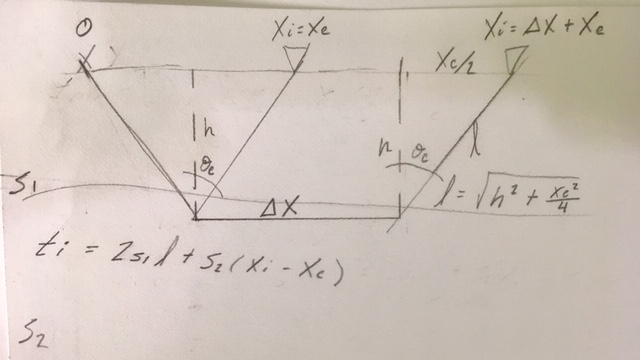
\includegraphics[width = \textwidth]{RefractionModel.jpg}
    \caption{A subsurface earth model for a raypath traveling through a homogeneous overburden layer and refracting along the half-space boundary. }
    \label{fig:refract}
\end{figure}
\FloatBarrier
\vspace{-15pt}
\subsection*{(a \& g \& h). Find the least squares and 1-norm estimates}
For the model parameters $t_0$ and $s_2$ plot the data, the fitted model, and the residuals. Report symmetric 95\% confidence intervals on the 1-norm solution.
\vspace{-1pt}
\begin{figure}[!h]
\begin{minipage}{0.5\linewidth}
\begin{equation}
    \mathbf{m_{L2}} = \left[
    \begin{array}{c}
      t_0 = 1.3357  \\
        s_2 = 0.25839 
    \end{array}\right]
\end{equation}
\end{minipage}%
\begin{minipage}{0.5\linewidth}
\begin{equation}
    \mathbf{m_{L1}} = \left[
    \begin{array}{c}
        t_0 = 2.0634  \\
         s_2 = 0.21316 
    \end{array}\right]
\end{equation}
\end{minipage}
\end{figure}

\begin{figure}[b]
    \centering
    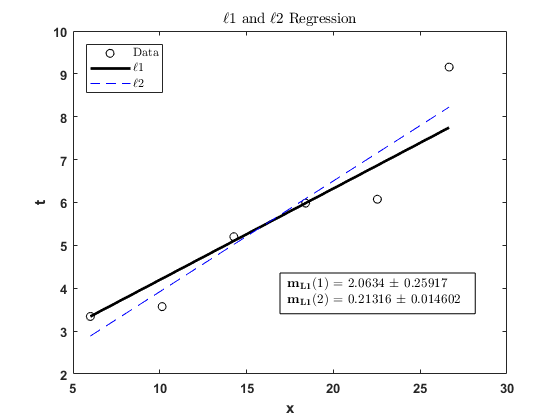
\includegraphics[width = .875\textwidth]{linearmodel_l1l2.png}
    \caption{The $\ell _1$ and $\ell _2$ parameter estimation of the seismic refraction problem. Symmetric 95\% confidence intervals found by Monte Carlo error propagation are listed for the $\ell_1$ parameters.}
    \label{fig:regression}
\end{figure}

\begin{figure}[t]
    \centering
    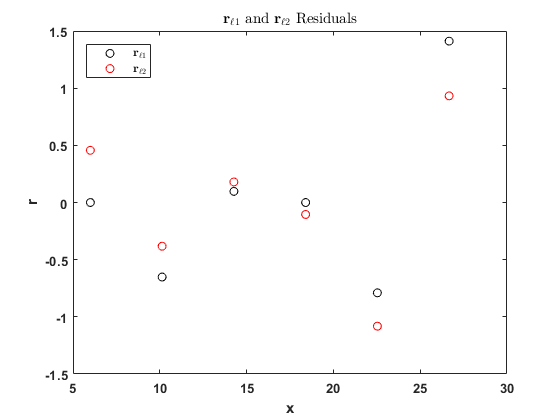
\includegraphics[width = .875\textwidth]{residuals_l1l2.png}
    \caption{The data residuals $(\mathbf{d - Gm})$ for the $\ell _1$ and $\ell _2$ parameter estimation.}
    \label{fig:residuals}
\end{figure}
\FloatBarrier
%\vspace{-40pt}
\subsection*{(b \& c). Calculate and comment on the model parameter correlation matrix and plot the error ellipsoid.}
$ \rho (m 1, m 2)=-0.9179 $ shows that the two parameters are highly negatively correlated and as result it is expected that the projection would be needle like with its long principal axis having a negative slope. This relationship is visualized in Figure \ref{fig:ellipsoid}.

\begin{figure}[p]
    \centering
    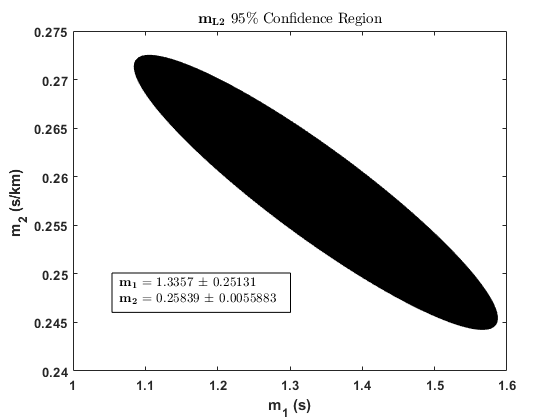
\includegraphics[width = .875\textwidth]{ml2_confidenceRegion.png}
    \caption{The conservative 95\% confidence region for the $\mathbf{m_{L2}}$ solution for $t_0$ and $s_2$. }
    \label{fig:ellipsoid}
\end{figure}
%\FloatBarrier
%\vspace{-40pt}
\subsection*{(e). Evaluate the value of $\chi^2$ for 1000 Monte Carlo simulations using the data prediction from the noise perturbed model.}

The experimental and theoretical probability distributions are compared in Figure \ref{fig:X2}. According the the $\chi$ \textit{by eye} test, the experiment agrees with the theory.
\begin{figure}[p]
    \centering
    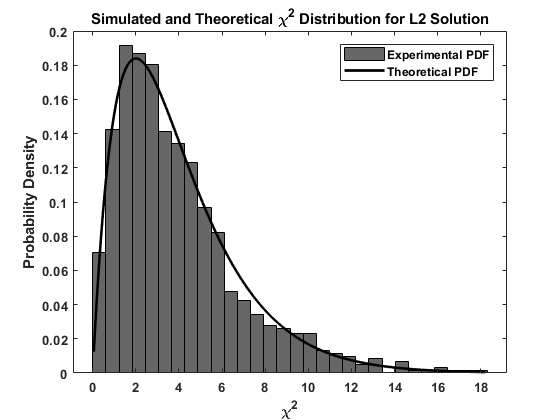
\includegraphics[width =.875 \textwidth]{X2pdf.png}
    \caption{The theoretical probability density function agrees ($\chi$ by eye) with the experimental distribution. }
    \label{fig:X2}
\end{figure}
%\FloatBarrier

\subsection*{(d \& f). Evaluate the p-value for the model, is the $\chi^2$ test consistent with the theoretical modeling and the data set?}
We retrieve a p-value of exactly $0$, which leads us to believe that the physical model is incorrect. ``A two-layer flat Earth structure gives the mathematical model

\begin{equation}
t_i = t_0 + s_2x_i
\label{eqn:ti}
\end{equation}
where the intercept time $t_0$ depends on the thickness and slowness of the upper layer, and $s_2$ is the slowness of the lower layer". Equation \ref{eqn:ti} represents a direct-wave approximation to the refracted raypath which is approximately correct for $x_i >> h$. This model is under parameterized with respect to the physics, leading to an undetermined problem that the bulk term $t_0$ does not adequately resolve. A more correct statement of the refraction model is
\begin{equation}
t_i = 2s_1\ell+ s_2(x_i-x_c)
\label{eqn:newti}
\end{equation}
where 
\begin{equation}
    \ell = \sqrt{h^2 + \frac{x_c^2}{4}}
\end{equation}
depends on the layer thickness $(h)$ and the critical distance $(x_c)$ for refraction 
\begin{equation}
    x_c = 2h \operatorname{tan}\theta _c
\end{equation}
and $\theta _c$, the critical angle for refraction, follows from Snell's Law
\begin{equation}
    \operatorname{sin}\theta_c = \frac{s_2}{s_1}.
\end{equation}

This formulation obviates the nested parameters that are required to accurately model a basic seismic refraction for a simple Earth model. Figure \ref{fig:refract} is the diagram of the refraction model that results in the travel-time equation (\ref{eqn:newti}). 

An independent estimate of $s1$ is required to solve (\ref{eqn:newti}). Typically the first arrival data include information for $x_i < x_c$ such that the direct-wave equation 
\begin{equation}
t_i = t_0 + s_1x_i
\label{eqn:t1}
\end{equation}
can be applied independently of equation \ref{eqn:newti}. These travel-time graphs typically display the cross-over distance 
\begin{equation}
    x_x = 2 h \sqrt{\frac{v_{2}+v_{1}}{v_{2}-v_{1}}}
\end{equation}
which depends on the overburden thickness $(h)$, and indicates which $x_i$ can be leveraged to estimate $s_1$. Additional arrival time information for $x_i < x_x$ is required for a unique solution of equation \ref{eqn:newti}.

\subsection*{(i). Discuss potential data outliers}
In order to find data that are statistical outliers we conducted a \textit{leave one out} analysis by excluding datum $i$ and recalculating the the 1-norm and 2-norm solution. Then the $\ell_1$-norm of the residuals corresponding to each iteration of the analysis is computed. Utilizing $t-$distribution (due to limited amount of observations), the 95\% confidence intervals of the 1-norm residuals of ${m_{L1}}$ and ${m_{L2}}$ estimates are calculated. The 95\% confidence intervals of both ${m_{L1}}$ and ${m_{L2}}$ indicate that datum $i=6$ is an outlier. This method is corroborated by inspection of Figure \ref{fig:regression}. It can be seen that the $\ell_1$ solution steers the regression line away from $(x_6,t_6)$. This indicates that the 1-norm solution, estimated by IRLS algorithm, considers this datum as an outlier.

\newpage
\section*{Exercise 5}
For the model equation $y_i = a_0 + a_1x_i + a_2x_i^2 .... a_{19}x_i^{19}$ and the given data, we found the following a parameters:

%% not sure what the best way is to display a long 
%% vector of numbers in latex.... 
\begin{center}
a = [ 0.000e+00,  1.082e+00, -1.000e-03, -4.700e-01,  3.000e-03,
    2.188e+00, -8.000e-03, -4.798e+00,  9.000e-03,  4.823e+00,
    -4.000e-03, -2.407e+00, -0.000e+00,  8.100e-01,  3.000e-03,
    -3.140e-01, -3.000e-03,  1.260e-01,  1.000e-03, -1.300e-02]
\end{center}

The parameter $a_1$ is in fact very close to 1 as it should be, since the data supplied are perfectly linear with a slope of 1 (i.e. y=x). The least squares solution is slightly wrong (1.082 versus 1) because the model that we are fitting does not describe the relationship between the data appropriately. 


\begin{figure}[!h]
    \centering
    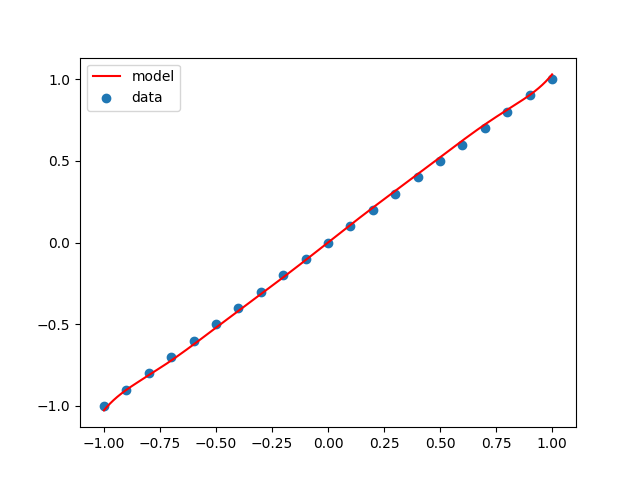
\includegraphics[width = .875\textwidth]{Ch2_Problem5.png}
    \caption{The over parameterized least squares fit to an exact linear equation.}
    \label{p5}
\end{figure}






\newpage
\section*{Appendix}
\subsection*{MATLAB Code used to answer Excercise 1.}
\begin{minted}{matlab}
% make sure we have a clean environment
clear
rand('state',0);
randn('state',0)
addpath 'C:\Users\snowfield\Desktop\Backup\Math\Inverse Theory\PEIP-code\Lib';

% Generate the x and y valuesy
t = [3.493500000000000;4.285300000000000;5.137400000000000;5.818100000000000;6.863200000000000;8.184100000000000];
x = [6;10.133300000000000;14.266700000000000;18.400000000000000;22.533300000000000;26.666700000000000];
ytrue = t;
N=length(x);
sig = 0.1;
sigma=sig*ones(N,1);
y = ytrue+sig*randn(size(x)).*ytrue;

% Build the matrix
G=[ones(size(x)) x];

% Apply the weighting
yw = y./sigma;
Gw = G./[sigma,sigma];

% Solve for the least-squares solution
disp('least-squares solution')
m2 = Gw\yw

% Solve for the 1-norm solution
disp('1-norm solution')
m1 = irls(Gw,yw,1.0e-5,1.0e-5,1,125)

% comute modeled
ymod1 = G * m1;
ymod2 = G * m2;

%% Plots
%  1. Data and fitted line.
%  2. residuals.
figure(1)
clf
plot(x,y,'ko');
hold on
p = plot(x,ymod1,'k',x,ymod2,'b--');
p(1).LineWidth = 2;
%%p(2).Marker = '*';
%%plot();
xlabel('x');
ylabel('t');
title('$\ell 1$ and $\ell 2$ Regression','interpreter','latex');
legend({'Data','$\ell 1$','$\ell 2$'},'Interpreter','latex','location','northwest')
set(gca,'fontweight','bold')

disp('Displaying Data and Linear Regression Line (fig 1)')


figure(2)
clf
plot(x,y-ymod1,'ko');hold on
plot(x,y-ymod2,'ro');
xlabel('x');
ylabel('r');
title('$\mathbf{r}_{\ell 1}$ and $\mathbf{r}_{\ell 2}$ Residuals','interpreter','latex')
legend({'$\mathbf{r}_{\ell 1}$','$\mathbf{r}_{\ell 2}$'},'Interpreter','latex','location','northwest')
set(gca,'fontweight','bold')



disp('Displaying Model Residuals vs. x (fig 2)');
%%
% Get the covariance matrix
ginv = inv(Gw'*Gw)*Gw';

disp('Covariance matrix')
covm = ginv*ginv'

% Find the parameter correlations
s=sqrt(diag(covm))

disp('correlation matrix')
r = covm./(s*s')

% Output covm and the eigenvalues/eigenvectors of covm.
disp('Covariance matrix for fitted parameters.')
covm

disp('Eigenvalues/eigenvectors of the covariance matrix');
[u,lam]=eig(inv(covm))
disp('95% confidence ellipsoid semiaxis lengths');
semi_axes = [sqrt(chi2inv(0.95,2)*(1./diag(lam)))]'
disp('95% confidence ellipsoid semiaxes')

[semi_axes(1)*u(:,1), semi_axes(2)*u(:,2)]

%
% Plot the 95% error ellipses for each pair of parameters
% Note that because we're doing pairs of parameters there are 2
% degrees of freedom in the Chi-square here, rather than 3.  
%
%generate a vector of angles from 0 to 2*pi
theta=(0:.01:2*pi)';
delta=sqrt(chi2inv(0.95,2));
%the radii in each direction from the center
r=zeros(length(theta),2);

figure(3)
clf

% compute the data for the m1, m2 ellipsoid.
C=covm((1:2),(1:2));
[u,lam]=eig(inv(C));
%calculate the x component of the ellipsoid for all angles
r(:,1)=(delta/sqrt(lam(1,1)))*u(1,1)*cos(theta)+(delta/sqrt(lam(2,2)))*u(1,2)*sin(theta);
%calculate the y component of the ellipsoid for all angles
r(:,2)=(delta/sqrt(lam(1,1)))*u(2,1)*cos(theta)+(delta/sqrt(lam(2,2)))*u(2,2)*sin(theta);

% plot the data for the m1, m2 ellipsoid
plot(m2(1)+r(:,1),m2(2)+r(:,2),'k');
fill(m2(1)+r(:,1),m2(2)+r(:,2),'k');

xlabel('m_1 (s)');
ylabel('m_2 (km)');
title('$\mathbf{m_{L2}}$ 95\% Confidence Region','interpreter','latex');
dim = [.2 .05 .3 .3];
str = {['$\mathbf{m_{1}} =$ ',num2str(m2(1)), ' $\pm$ ', num2str(semi_axes(1))],['$\mathbf{m_{2}} =$ ',num2str(m2(2)), ' $\pm$ ', num2str(semi_axes(2))]};
annotation('textbox',dim,'String',str,'FitBoxToText','on','interpreter','latex');
set(gca,'fontweight','bold')
%%
% Because there are 2 parameters to estimate, we have N-2 degrees
% of freedom.
%
dof = N-2;
disp(['Chi-square misfit for ',num2str(dof),' dof'])
chi2 = norm((y - G*m2)./sigma)^2

% Find the p-value for this data set
disp('chi-square p-value')
p = 1-chi2cdf(chi2,dof)

% Monte Carlo Section
y0 = G*m2; 

for nreal = 1:1000
  % Generate a trial data set of perturbed, weighted data
  ytrial = y0+sigma.*randn(N,1);
  ywtrial=ytrial./sigma;
  mmc(nreal,:)=(Gw\ywtrial)';
  chimc(nreal)= norm((G*mmc(nreal,:)'-ytrial)./sigma)^2;
end
% Calculate the Theoretical X^2 pdf
chi = chi2pdf(linspace(min(chimc),max(chimc),1000),dof);
% chi = chi2pdf(mmc,dof);


% Plot the histogram of chi squared values
figure(4)
clf
histogram(chimc,30,'FaceColor','k','normalization','pdf');
hold on;
plot(linspace(min(chimc),max(chimc),1000),chi,'k','linewidth',2)
ylabel('Probability Density');
xlabel('\chi^2')
title('Simulated and Theoretical \chi^2 Distribution for L2 Solution');
legend('Experimental PDF','Theoretical PDF')
set(gca,'fontweight','bold')

%%
% Monte Carlo Section for the 1-norm model
% The 1-norm estimated data
y01 = G*m1; 

nreal=1000;

disp('generating Monte Carlo realizations');
%generate the nreal Monte Carlo solutions
for j = 1:nreal
  % Generate a trial data set of perturbed, weighted data
  ytrial = y01+sigma.*randn(N,1);
  ywtrial=ytrial./sigma;
  
  % Store the 1-norm parameters and misfit
  mmc(j,:)=irls(Gw,ywtrial,1.0e-5,1.0e-5,1,500)';
  chimc(j)= norm((G*mmc(j,:)'-y01)./sigma)^2;
end

% figure out how many Monte Carlo points are in the %95 confidence region
disp('confidence interval inclusion check (should be about 0.95):') 
nnz(chimc<=chi2inv(.95, dof))/nreal

% Calculate the covariance of the parameters in the realizations
disp('Emperical covariance of m1 models');
covmemp=mmc-ones(nreal,1)*mean(mmc);
covmemp=(covmemp'*covmemp)/nreal

% Get the 1.96-sigma (95%) conf intervals
disp('95% parameter confidence intervals (m-, mest, m+) on 1-norm solution')
del = 1.96*sqrt(diag(covmemp));
[m1-del , m1 , m1+del]
figure(1);
dim = [.5 .05 .3 .3];
str = {['$\mathbf{m_{L1}}(1) =$ ',num2str(m1(1)), ' $\pm$ ', num2str(del(1))],['$\mathbf{m_{L1}}(2) =$ ',num2str(m1(2)), ' $\pm$ ', num2str(del(2))]};
annotation('textbox',dim,'String',str,'FitBoxToText','on','interpreter','latex');
%% contributions from each of the data points to the 1-norm misfit measure
 
for i = 1:N
    xnew = x;
    tnew = t;
    xnew(i) = [];
    tnew(i) = [];
    ytrueNew = tnew;
    Nnew=length(xnew);
    sigmanew=sig*ones(Nnew,1);
    ynew = ytrueNew+sig*randn(size(xnew)).*ytrueNew;

    % Build the matrix
    Gnew=[ones(size(xnew)) xnew];

    % Apply the weighting
    ywnew = ynew./sigmanew;
    Gwnew = Gnew./[sigmanew,sigmanew];

    % Solve for the least-squares solution
    disp('least-squares solution')
    m2new(i,:) = Gwnew\ywnew

    % Solve for the 1-norm solution
    disp('1-norm solution')
    m1new(i,:) = irls(Gwnew,ywnew,1.0e-5,1.0e-5,1,1)

    % comute modeled
    ymod1new(:,i) = Gnew * m1new(i,:)';
    ymod2new(:,i) = Gnew * m2new(i,:)';
    
    % compute residuals
    r1(:,i) = ynew - ymod1new(:,i);
    r2(:,i) = ynew - ymod2new(:,i);
    
    % compute norm1 of residuals
    nr1(1,i) = norm(r1(:,i),1);
    nr2(1,i) = norm(r2(:,i),1);

end

figure(5)
clf
plot(1:N,nr1,'ko');
hold on
plot(1:N,nr2,'ro');
xlabel('Data points');
ylabel('norm1 of Residuals');
title('$\mathbf{r}_{\ell 1}$ and $\mathbf{r}_{\ell 2}$ Residuals','interpreter','latex')
legend({'$\mathbf{r}_{\ell 1}$','$\mathbf{r}_{\ell 2}$'},'Interpreter','latex','location','northwest')
set(gca,'fontweight','bold')


%%%%%%%%% confidence interval and data outliers %%%%%%%%%%%%%%%%%%%

con1 = [mean(nr1) - (tinv(0.975,5)*std(nr1)/(6^0.5)), mean(nr1) + (tinv(0.975,5)*std(nr1)/(6^0.5))];
con2 = [mean(nr2) - (tinv(0.975,5)*std(nr2)/(6^0.5)), mean(nr2) + (tinv(0.975,5)*std(nr2)/(6^0.5))];    
for i = 1:6
    if (nr1(1,i) > con1(1,2) || nr1(1,i) < con1(1,1))
        disp(['Data rank number ', num2str(i), ' acording to norm1 of mL1 estimate is an outlier'])
    end
end
for i = 1:6
    if (nr2(1,i) > con2(1,2) || nr2(1,i) < con2(1,1))
        disp(['Data rank number ', num2str(i), ' acording to norm1 of mL2 estimate is an outlier'])
    end
end

\end{minted}
\newpage
\subsection*{Python Code used to answer excercise 2.}
\begin{minted}{python}
import numpy as np
from matplotlib import pyplot as plt
#
# Ga = y 
m = 21
n = 20
G = np.ones((m,n))

y = np.ones(m)
x = np.linspace(-1,1,m)

# form the G matrix 
G[:,0] = 1  # the first column (corresponding w/ a0) is 1

# loop through the rows of G 
for i in range(m):
    G[i,:]=np.array([x[i]**k for k in range(n)]) # each row is [1 ax_i**1 .... ax_i**19]

# solve for the ml2 solution
GTG = np.dot(G.T,G) # form G^TG
invGTG= np.linalg.inv(GTG)
mL2 = np.dot(np.dot(invGTG, G.T), y)


# create a fine grid to plot fitted polynomial 
# on the range x=[-1 , -.999 .... .999, 1] 
xFine = np.arange(-1,1,.001)
gFine = np.ones((xFine.shape[0], n))   # recall we have n=20 a parameters 
gFine[:,0] = 1
for i in range(gFine.shape[0]):
   gFine[i,:]=np.array([xFine[i]**k for k in range(n)]) # each row is [1 ax_i**1 .... ax_i**19]


# plot the original data
plt.scatter(x,y, label='data')
plt.plot(xFine, np.dot(gFine,mL2), label='model', color='red')
plt.legend()
plt.savefig("Ch2_Problem5")
\end{minted}



\end{document}

